\chapter{Supporting materials for flexible diffusion on varying dimensionality data}

\section{Training objective}
\label{sec:tddm-ApdxTrainingObjective}
We estimate our objective $\mathcal{L}_\text{JD}(\theta)$ by taking minibatches from the expectation 
\begin{equation}
    \mathcal{U}(t; 0, T) q_{0,t}(\mX_0, \mX_t, M_t) \delidxdist(i | n_t) \updelta_{\text{del}(\mX_t, i)}(\mV).
\end{equation}
We first sample $t \sim \mathcal{U}(0, T)$ and then take samples from our dataset $\mX_0 \sim \pdata(\cdot)$. In order to sample $q_{t|0}(\mX_t, M_t | \mX_0)$ we need to add noise, delete dimensions, and sample a mask variable. When the Gaussian noising process is isotropic, we can add a suitable amount of noise to all dimensions of $\mX_0$ and then delete dimensions of that noised full dimensional value. More specifically, we first sample $\tilde{\mX}_t = (n_0, \tilde{\rvx}_t)$ with $\tilde{\rvx}_t \sim \mathcal{N}(\tilde{\rvx}_t; \alpha(t) \rvx_0, \sigma(t)^2 I_{n_0 d})$. Then we sample the number of dimensions to delete. This is simple to do when our rate function is independent of $n$ except for the case when $n=1$ at which it is zero. We simply sample a Poisson random variable with mean parameter $\int_0^t \forwardrate_s \rmd s$ and then clamp its value such that the maximum number of possible components that are deleted is $n_0 - 1$. This gives the appropriate distribution over $n$, 
\begin{equation}
    q_{t|0}(n | n_0) = \begin{cases}
         \frac{(\int_0^t \forwardrate_s \rmd s)^{n_0 - n}}{(n_0 - n)!} \text{exp}(- \int_0^t \forwardrate_s \rmd s)&\textstyle  1 < n \leq n_0 \\
        1 -  \sum_{m=2}^{n_0} \frac{(\int_0^t \forwardrate_s \rmd s)^{n_0 - m}}{(n_0 - m)!} \text{exp}(- \int_0^t \forwardrate_s \rmd s)  &\textstyle  n = 1.
    \end{cases}
\end{equation}
To sample which dimensions are deleted, we can sample $\delidxdist(i_1 | n_0) \delidxdist(i_2 | n_0-1) \dots \delidxdist(i_{n_0 - n_t} | n_t+1)$ from which we can create the mask $M_t$ and apply it to $\tilde{\mX}_t$ to obtain $\mX_t = M_t(\tilde{\mX}_t)$. When $\delidxdist(i | n) = 1/n$ this is especially simple to do by simply randomly permuting the components of $\tilde{\mX}_t$, and then removing the final $n_0 - n_t$ components. Similarly, if $\delidxdist(i | n)$ is defined to always delete the final component, this will deterministically result in a mask that always removes the final $n_0 - n_t$ components.

We use the $\epsilon$-prediction parameterisation described in \cref{sec:diffusion-training}, parameterising $\rvs_\theta$ in terms of a noise prediction network that predicts $\epsilon$ where $\rvx_t = \alpha(t) M_t(\rvx_0) + \sigma(t) \cdot \epsilon$ with $\epsilon \sim \mathcal{N}(0, I_{n_t d})$. We set the weighting function such that $\lambda^\epsilon(t)/u(t) = 1$ as in the uniform weighting approach used by \citet{song2020score}. Our objective to learn $\rvs_\theta$ then becomes
\begin{equation}
    - \mathbb{E}_{\mathcal{U}(t; 0, T) \pdata(\mX_0) q_{t|0}(M_t, n_t | \mX_0) \mathcal{N}(\epsilon; 0, I_{n_t d})} \left[ \norm{\hat{\mathbf{\epsilon}}_\theta(\mX_t, t) - \epsilon}^2 \right]
\end{equation}
with $\rvx_t = \alpha(t) M_t(\rvx_0) + \sigma(t) \epsilon$, $\rvs_\theta(\mX_t, t) = \frac{-1}{\sigma(t)} \hat{\mathbf{\epsilon}}_\theta(\mX_t, t)$.

Further, by using the parameterisation given in Proposition \ref{prop:backwardrateparam}, we can directly supervise the value of $p_{0|t}^\theta(n_0 | \mX_t)$ by adding an extra term to our objective. We can treat the learning of $p_{0|t}^\theta(n_0 | \mX_t)$ as a standard prediction task where we aim to predict $n_0$ given access to $\mX_t$. A standard objective for learning $p_{0|t}^\theta(n_0 | \mX_t)$ is then the cross entropy
\begin{equation}
    \underset{\theta}{\text{max}} \quad \mathbb{E}_{q_{0,t}(\mX_0, \mX_t)} \left[ \log p_{0|t}^{\theta}(n_0 | \mX_t) \right] .
\end{equation}
Our augmented objective then becomes
\begin{align} \label{eq:augmentedObjective}
    \tilde{\mathcal{L}}_\text{JD}(\theta) = &T\mathbb{E} [ -\frac{1}{2}\norm{\hat{\mathbf{\epsilon}}_\theta(\mX_t, t) - \epsilon}^2 - \backwardrate_t^\theta(\mX_t) + \forwardrate_t(n_t) \log \backwardrate_t^\theta(\mV) \\ 
    &+ \forwardrate_t(n_t) \log \autonet_t^\theta(\xadd_t, i | \mV) + \gamma \cdot \log p_{0|t}^\theta (n_0 | \mX_t) ] \nonumber
\end{align}
where the expectation is taken with respect to 
\begin{equation}
\mathcal{U}(t; 0, T) \pdata(\mX_0) q_{t|0}(M_t, n_t | \mX_0) \mathcal{N}(\epsilon; 0, I_{n_t d}) \delidxdist(i | n_t) \updelta_{\text{del}(\mX_t, i)}(\mV)
\end{equation}
with $\rvx_t = \alpha(t) M_t(\rvx_0) + \sigma(t) \epsilon$ and $\gamma$ being a scalar hyperparameter which weights the cross entropy loss.


\section{Experimental details}
\label{sec:tddm-ExperimentDetails}
The code corresponding to \cref{ch:tddm} is available at \url{https://github.com/andrew-cr/jump-diffusion}.

\subsection{Molecules}

\subsubsection{Network architecture}
\paragraph{Backbone}
For our backbone network architecture, we used the EGNN used in \citet{hoogeboom2022equivariant}. This is a specially designed graph neural network applied to the point cloud treating it as a fully connected graph. A special equivariant update is used, operating only on distances between atoms. We refer to \citet{hoogeboom2022equivariant} for the specific details on the architecture. We used the same network size as \citet{hoogeboom2022equivariant}'s QM9 experiments; in particular it has $9$ layers with a hidden node feature size of $256$. The output of the EGNN is fed into a final output projection layer to give the score network output $\rvs_\theta(\mX_t, t)$.

\paragraph{Component number prediction}
To obtain $p_{0|t}^\theta(n_0 | \mX_t)$,  we take the embedding produced by the EGNN before the final output embedding layer and pass it through 8 transformer layers each consisting of a self-attention block and an MLP block applied channel wise. Our transformer model dimension is $128$ and so we project the EGNN embedding output down to $128$ before entering into the transformer layers. We then take the output of the transformer and take the average embedding over all nodes. This embedding is then passed through a final projection layer to give softmax logits over the $p_{0|t}^\theta(n_0 | \mX_t)$ distribution.

\paragraph{Autoregressive distribution}
Our $\autonet_t^\theta(\yadd, i | \mX_t)$ network has to predict the position and features for a new atom when it is added to the molecule. Since the point cloud is permutation invariant, we do not need to predict $i$ and so we just need to parameterise $\autonet_t^\theta(\yadd | \mX_t)$. We found the network to perform the best if the network first predicts the nearest atom to the new atom and then a vector from that atom to the location of the new atom. To achieve this, we first predict softmax logits for a distribution over the nearest atom by applying a projection to the embedding output from the previously described transformer block. During training, the output of this distribution can be directly supervised by a cross entropy loss. Given the nearest atom, we then need to predict the position and features of the new atom to add. We do this by passing in the embedding generated by the EGNN and original point cloud features into a new transformer block of the same size as that used for $p_{0|t}^\theta(n_0 | \mX_t)$. We also input the distances from the nearest atom to all other atoms in the molecule currently as an additional feature. To obtain the position of the new atom, we will take a weighted sum of all the vectors between the nearest atom and other atoms in the molecule. This is to make it easy for the network to create new atoms `in plane' with existing atoms which is useful for e.g. completing rings that have to remain in the same plane. To calculate the weights for the vectors, we apply an output projection to the output of the transformer block. The new atom features (atom type and charge) are generated by a separate output projection from the transformer block. For the position and features, $\autonet_t^\theta(\yadd | \mX_t)$ outputs both a mean and a standard deviation for a Gaussian distribution. For the position distribution, we set the standard deviation to be isotropic to remain equivariant to rotations. In total our model has around 7.3 million parameters.

\subsubsection{Training}
We train our model for 1.3 million iterations at a batch size of $64$. We use the Adam optimiser with learning rate $0.00003$. We also keep a running exponential moving average of the network weights that is used during sampling as is standard for training diffusion models~\citep{ho2020denoising, song2020score, karras2022elucidating} with a decay parameter of $0.9999$. We train on the 100K molecules contained in the QM9 training split. We model hydrogens explicitly. Training a model requires approximately $7$ days on a single GPU.

\citet{hoogeboom2022equivariant} encode the atom type as a one-hot vector and diffused as a continuous variable along with the positions and charge values for all atoms. They found that multiplying the one-hot vectors by $0.25$ to boost performance by allowing the atom-type to be decided later on in the diffusion process. We instead multiply the one-hot vectors by $4$ so that atom-type is decided early on in the diffusion process which improves our guided performance when conditioning on certain atom-types being present. We found our model is robust to this change and achieves similar sample quality to \citet{hoogeboom2022equivariant} as shown in \cref{tab:uncond_mol}.

When deleting dimensions, we first shuffle the ordering of the nodes and then delete the final $n_0 - n_t$ nodes. The cross entropy loss weighting in \cref{eq:augmentedObjective} is set to $1$.

Following \citet{hoogeboom2022equivariant} we train our model to operate within the centre of mass (CoM) zero subspace of possible molecule positions. The means, throughout the forward and reverse process, the average position of an atom is $0$. In our trans-dimensional framework, this is achieved by first deleting any atoms required under the forward component deletion process. We then move the molecule such that its CoM is $0$. We then add CoM free noise such that the noisy molecule also has CoM$=0$. Our score model $\rvs_\theta$ is parameterised through a noise prediction model $\hat{\mathbf{\epsilon}}_\theta$ which is trained to predict the CoM free noise that was added. Therefore, our score network learns suitable directions to maintain the process on the CoM$=0$ subspace. For the position prediction from $\autonet_t^\theta(\yadd | \mX_t)$ we train it to predict the new atom position from the current molecules reference frame. When the new atom is added, we then update all atom positions such that CoM$=0$ is maintained.

\subsubsection{Sampling}
During sampling we found that adding corrector steps~\citep{song2020score} improved sample quality. Intuitively, corrector steps form a process that has $p_t(\mX)$ as its stationary distribution rather than the process progressing toward $p_0(\mX)$. We use the same method to determine the corrector step size $\zeta$ as \citet{song2020score}. For the conditional generation tasks, we also found it useful to include corrector steps for the component generation process. As shown by \citet{campbell2022continuous}, corrector steps in discrete spaces can be achieved by simulating with a rate that is the addition of the forward and reverse rates. We achieve this in the context of trans-dimensional modelling by first simulating a possible insertion using $\backwardrate_t^\theta$ and then simulating a possible deletion using $\forwardrate_t$. We describe our overall sampling algorithm in \cref{alg:backwardsamplingWithCorrector}.

\begin{algorithm}
\begin{algorithmic}[1]
    \State $t \leftarrow T$
    \State $\mX \sim \mathbb{I}\{ n=1\} \mathcal{N}(\rvx; 0, I_{d})$
    \While{ $t > 0$}
    \State $u \sim \mathcal{U}(0, 1)$
    \If{$u < \backwardrate_{t}^\theta(\mX) \updelta t$}
    \State $\xadd, i \sim \autonet_{t}^\theta(\xadd, i | \mX)$
    \State $\mX \leftarrow \text{ins}(\mX, \xadd, i)$
    \EndIf
    \State  $\epsilon \sim \mathcal{N}(0, I_{nd})$
    \State $\rvx \leftarrow \rvx - \backwarddrift_{t}^\theta(\mX) \updelta t + g_{t} \sqrt{\updelta t} \epsilon$
    \For{$c = [1, \dots, C]$}
        \Comment{Corrector steps}
        \State $\epsilon \sim \mathcal{N}(0, I_{nd})$
        \State $\rvx \leftarrow \rvx + \zeta s_{t-\updelta t}^\theta(\mX) + \sqrt{2 \zeta} \epsilon$
        \State $u \sim \mathcal{U}(0, 1)$
        \If{$u < \backwardrate_{t-\updelta t}^\theta(\mX) \updelta t$}
        \State $\xadd, i \sim \autonet_{t-\updelta t}^\theta(\xadd, i | \mX)$
        \State $\mX \leftarrow \text{ins}(\mX, \xadd, i)$
        \EndIf
        \State $u \sim \mathcal{U}(0, 1)$
        \If{$u < \forwardrate_{t-\updelta t}(n) \updelta t$}
            \State $i \sim \delidxdist(i | n)$
            \State $\mX \leftarrow \text{del}(\mX, i)$
        \EndIf
    \EndFor
    \State $\mX \leftarrow (n, \rvx)$
    \State $t \leftarrow t - \updelta t$
    \EndWhile
\end{algorithmic}
\caption{Sampling from the generative process with $C$ corrector steps. The for loop marked ``Corrector steps'' is the only change from \cref{alg:backwardsampling}.}
\label{alg:backwardsamplingWithCorrector}
\end{algorithm}

\subsubsection{Evaluation}
\paragraph{Unconditional}
For our unconditional sampling evaluation, we start adding corrector steps when $t<0.1T$ in the backward process and use $5$ corrector steps without the corrector steps on the number of components. We set $\updelta = 0.05$ for $ t > 0.5T$ and $\updelta = 0.001$ for $t<0.5T$ such that the total number of network evaluations is $1000$. We show the distribution of sizes of molecules generated by our model in \cref{fig:tddm-uncond_dims} and show more unconditional samples in \cref{fig:tddm-apdxUncondMolSamples}. We find our model consistently generates realistic molecules and achieves a size distribution similar to the training dataset even though this is not explicitly trained and arises from sampling our reverse rate $\backwardrate_t^\theta$. Since we are numerically integrating a continuous time process and approximating the true time reversal rate $\backwardrate_t^*$, some approximation error is expected. For this experiment, sampling all of our models and ablations takes approximately $2$ GPU days on Nvidia $1080$Ti GPUs.

\paragraph{Conditional}
For evaluating applying conditional diffusion guidance to our model, we choose $10$ conditioning tasks that each result in a different distribution of target dimensions. The task is to produce molecules that include at least a certain number of target atom types. We then guide the first set of atoms generated by the model to have these desired atom types. The tasks chosen are given in \cref{tab:molecule_conditions}. Molecules in the training dataset that meet the conditions in each task have a different distribution of sizes. The tasks were chosen so that we have an approximately linearly increasing mean number of atoms for molecules that meet the condition. We also require that there are at least 100 examples of molecules that meet the condition within the training dataset.\\

For sampling when using conditional diffusion guidance, we use $3$ corrector steps throughout the reverse process with $\updelta t = 0.001$. For these conditional tasks, we include the corrector steps on the number of components. We show the distribution of dimensions for each task from the training dataset and from our generated samples in \cref{fig:tddm-apdx_CondDims}. Our metrics are calculated by first drawing 1000 samples for each conditioning task and then finding the Hellinger distance between the size distribution generated by our method (orange diagonal hashing in \cref{fig:tddm-apdx_CondDims}) and the size distribution for molecules in the training dataset that match the conditions of the task (green no hashing in \cref{fig:tddm-apdx_CondDims}). We find that indeed our model when guided by diffusion guidance can automatically produce a size distribution close to the ground truth size distribution found in the dataset for that conditioning value. We show samples generated by our conditionally guided model in \cref{fig:tddm-CondSampleExamples}. We can see that our model can generate realistic molecules that include the required atom types and are of a suitable size. For this experiment, sampling all of our models and ablations takes approximately $13$ GPU days on Nvidia $1080$Ti GPUs.

\paragraph{Interpolations}
For our interpolations experiments, we follow the set up of \citet{hoogeboom2022equivariant} who train a new model conditioned on the polarizability of molecules in the dataset. We train a conditional version of our model which can be achieved by simply adding in the polarizability as an additional feature input to our backbone network and re-using all the same hyperparameters. We show more examples of interpolations in \cref{fig:tddm-apdxMoreInterps}.


\begin{figure}
    \centering
    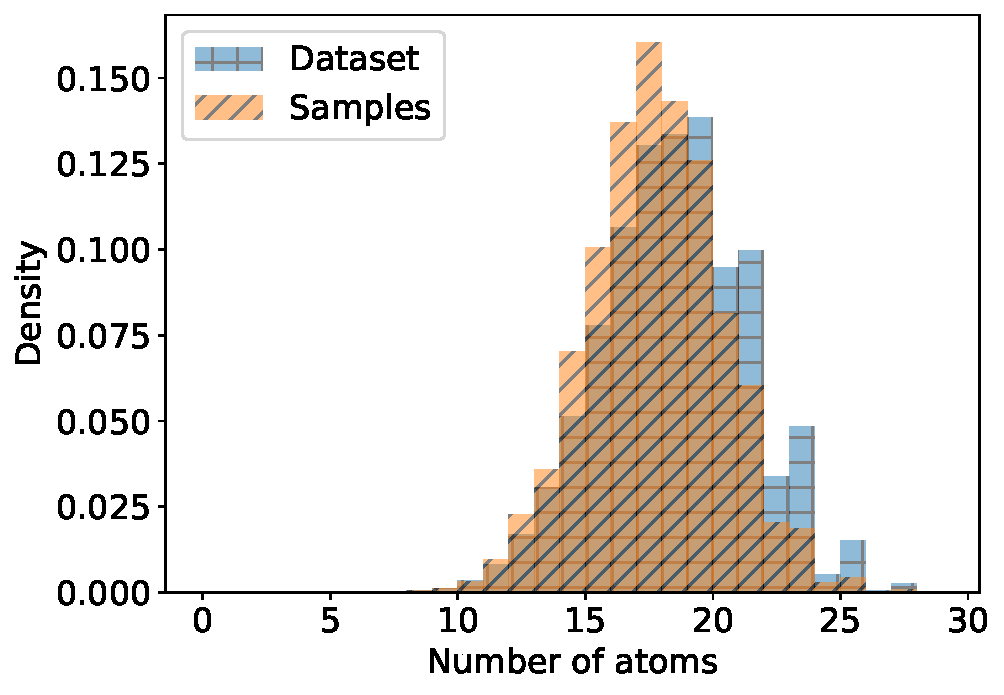
\includegraphics[width=8cm]{figs/tddm/uncond_dims.pdf}
    \caption{Distribution of the size of molecules in the QM9 dataset as measured through the number of atoms versus the distribution of the size of molecules generated by our unconditional model.}
    \label{fig:tddm-uncond_dims}
\end{figure}

\begin{figure}
    \centering
    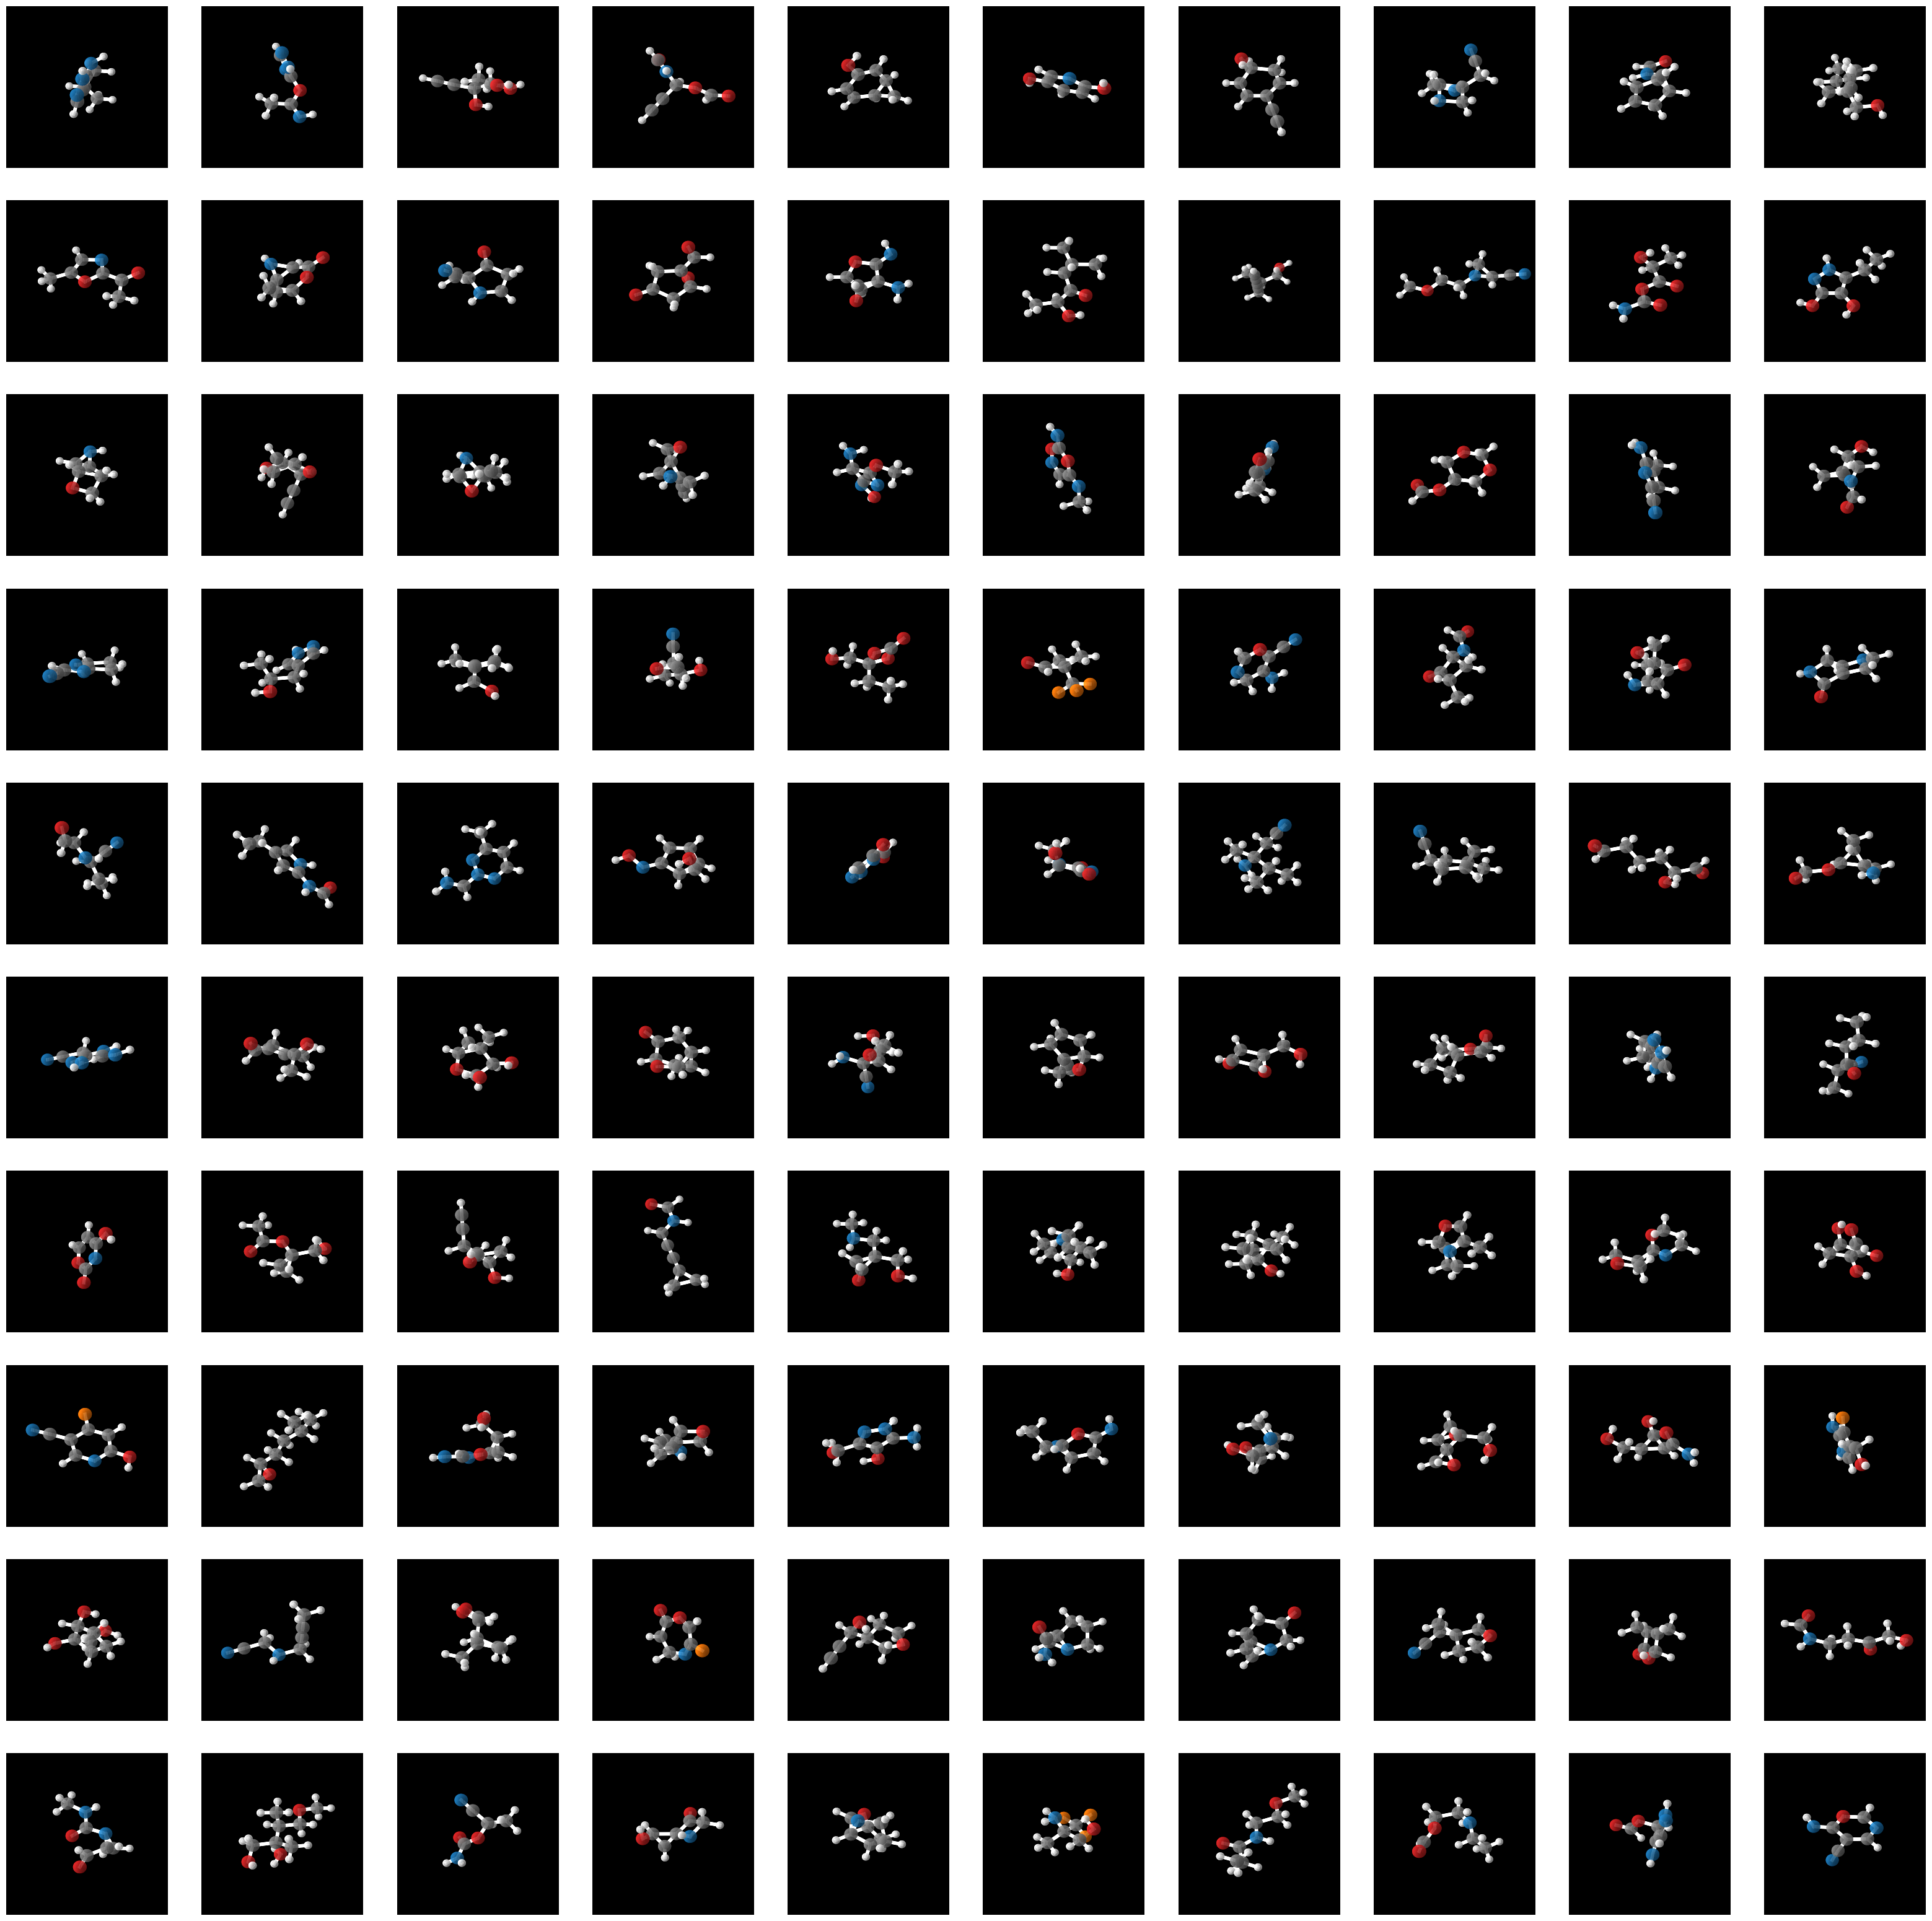
\includegraphics[width=\textwidth]{figs/tddm/uncond_samples_image_bright.png}
    \caption{Unconditional samples from our model.}
    \label{fig:tddm-apdxUncondMolSamples}
\end{figure}

\begin{table}[ht]
     \centering
   \caption{The 10 conditioning tasks used for evaluation. The number of each atom type required for the task is given in columns $2-5$ whilst the average number of atoms in molecules that meet this condition in the training dataset is given in the $6$th column.}
   \begin{tabular}{@{}lccccc@{}}
     \toprule
     Task & Carbon & Nitrogen & Oxygen & Fluorine & \shortstack{Mean Number \\ of Atoms} \\ \midrule
     1 & 4 & 1 & 2 & 1 & 11.9 \\
     2 & 4 & 3 & 1 & 1 & 13.0 \\
     3 & 5 & 2 & 1 & 1 & 13.9 \\
     4 & 6 & 0 & 1 & 1 & 14.6\\
     5 & 5 & 3 & 1 & 0 & 16.0\\
     6 & 6 & 3 & 0 & 0 & 17.2\\
     7 & 6 & 1 & 2 & 0 & 17.7\\
     8 & 7 & 1 & 1 & 0 & 19.1\\
     9 & 8 & 1 & 0 & 0 & 19.9\\
     10 & 8 & 0 & 1 & 0 & 21.0\\ \bottomrule
   \end{tabular}
   \label{tab:molecule_conditions}
\end{table}

\begin{figure}
    \centering
    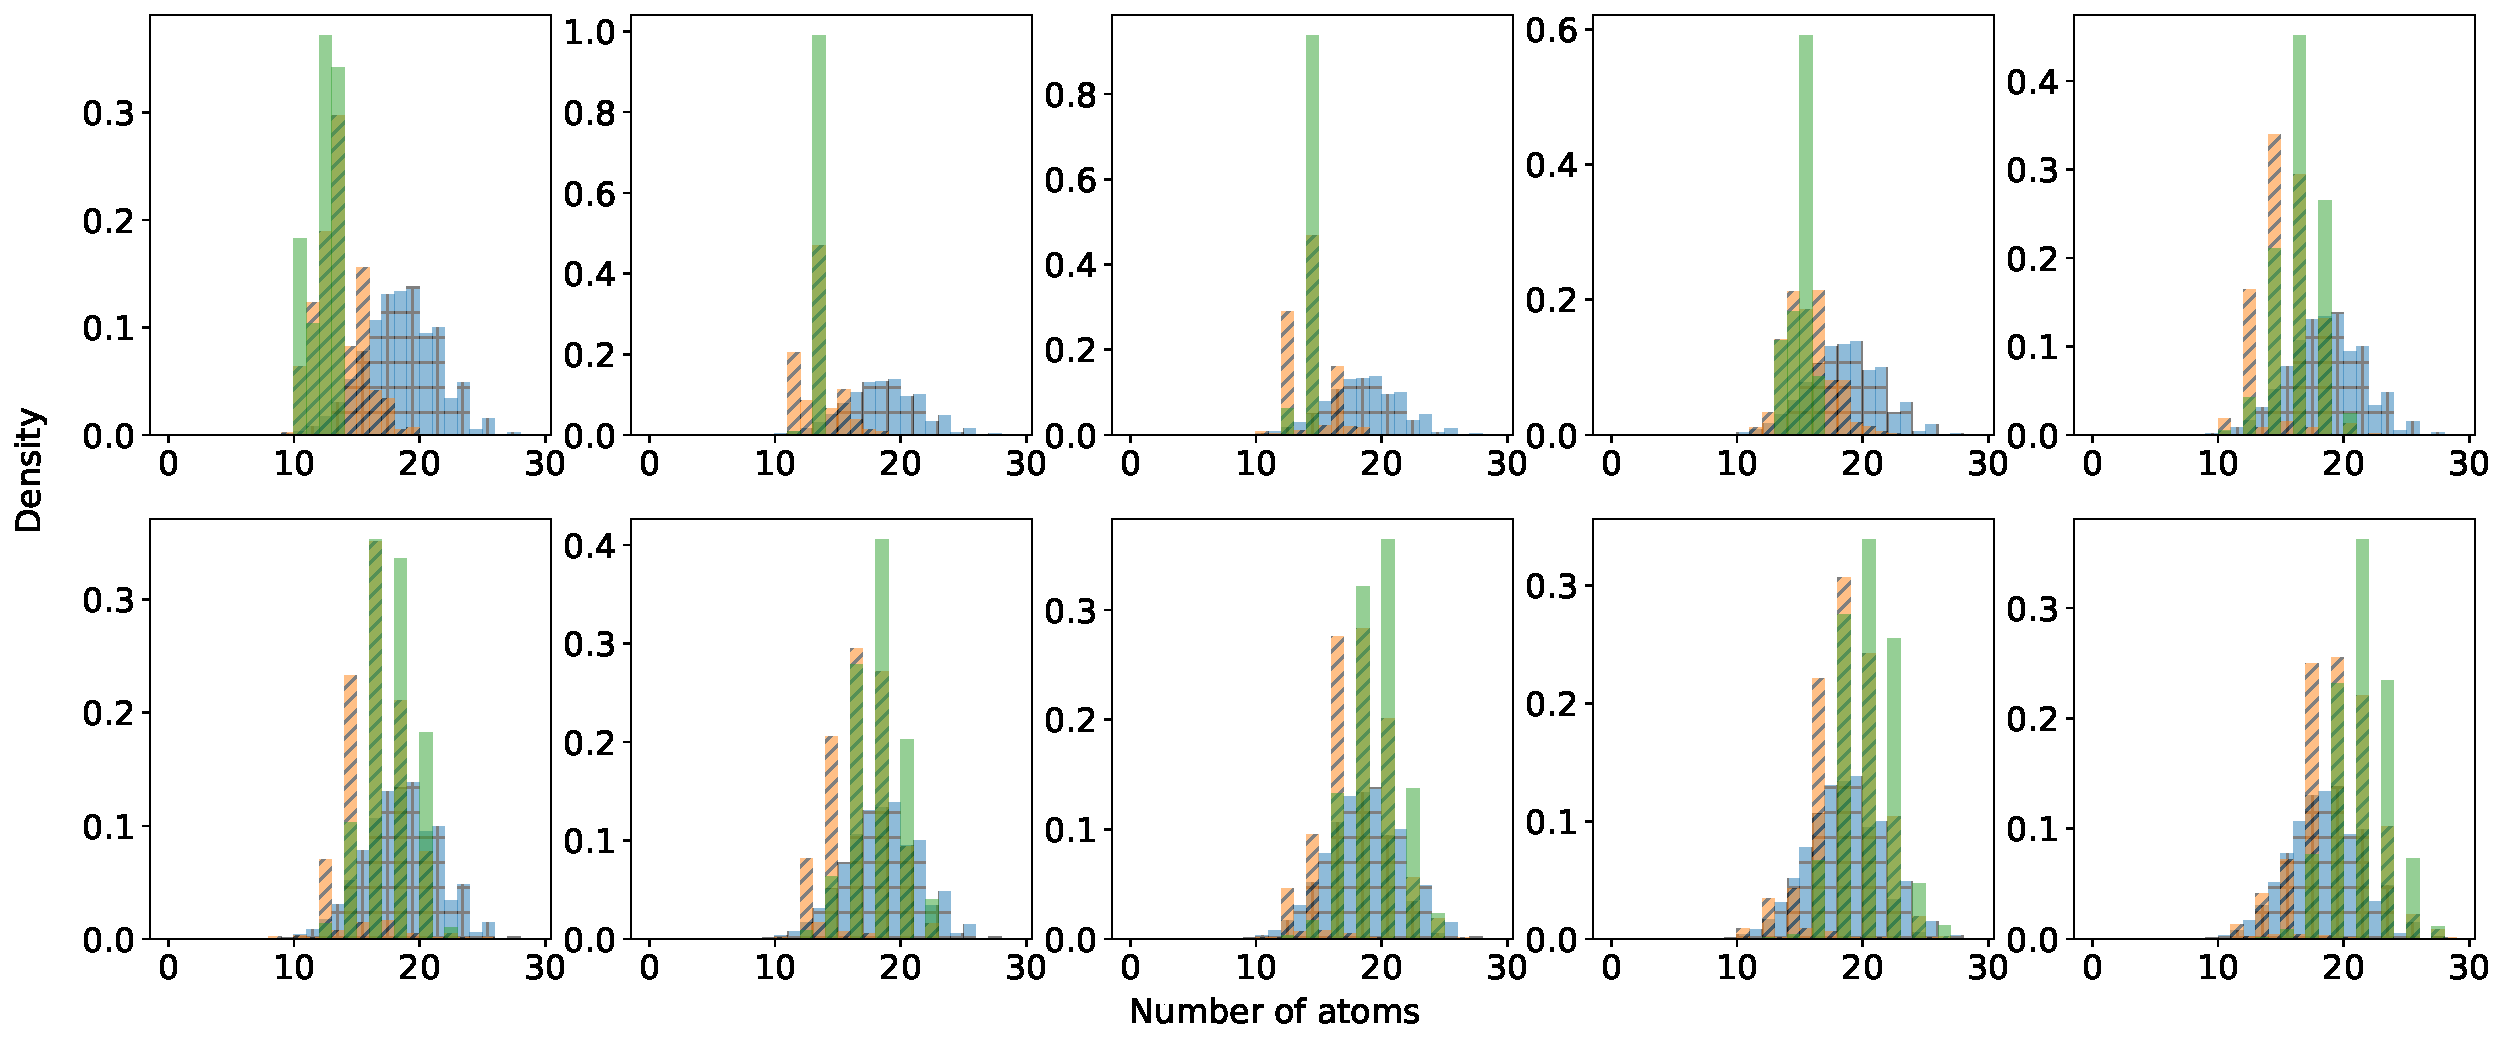
\includegraphics[width=\textwidth]{figs/tddm/cond_dims.pdf}
    \caption{Distribution of molecule sizes for each conditioning task. Tasks $1-5$ are shown left to right in the top row and tasks $6-10$ are shown left to right in the bottom row. We show the unconditional size distribution from the dataset in blue vertical/horizontal hashing, the size distribution of our conditionally generated samples in orange diagonal hashing and finally the size distribution for molecules in the training dataset that match the conditions of each task (the ground truth size distribution) in green no hashing.}
    \label{fig:tddm-apdx_CondDims}
\end{figure}



\begin{figure}
    \centering
    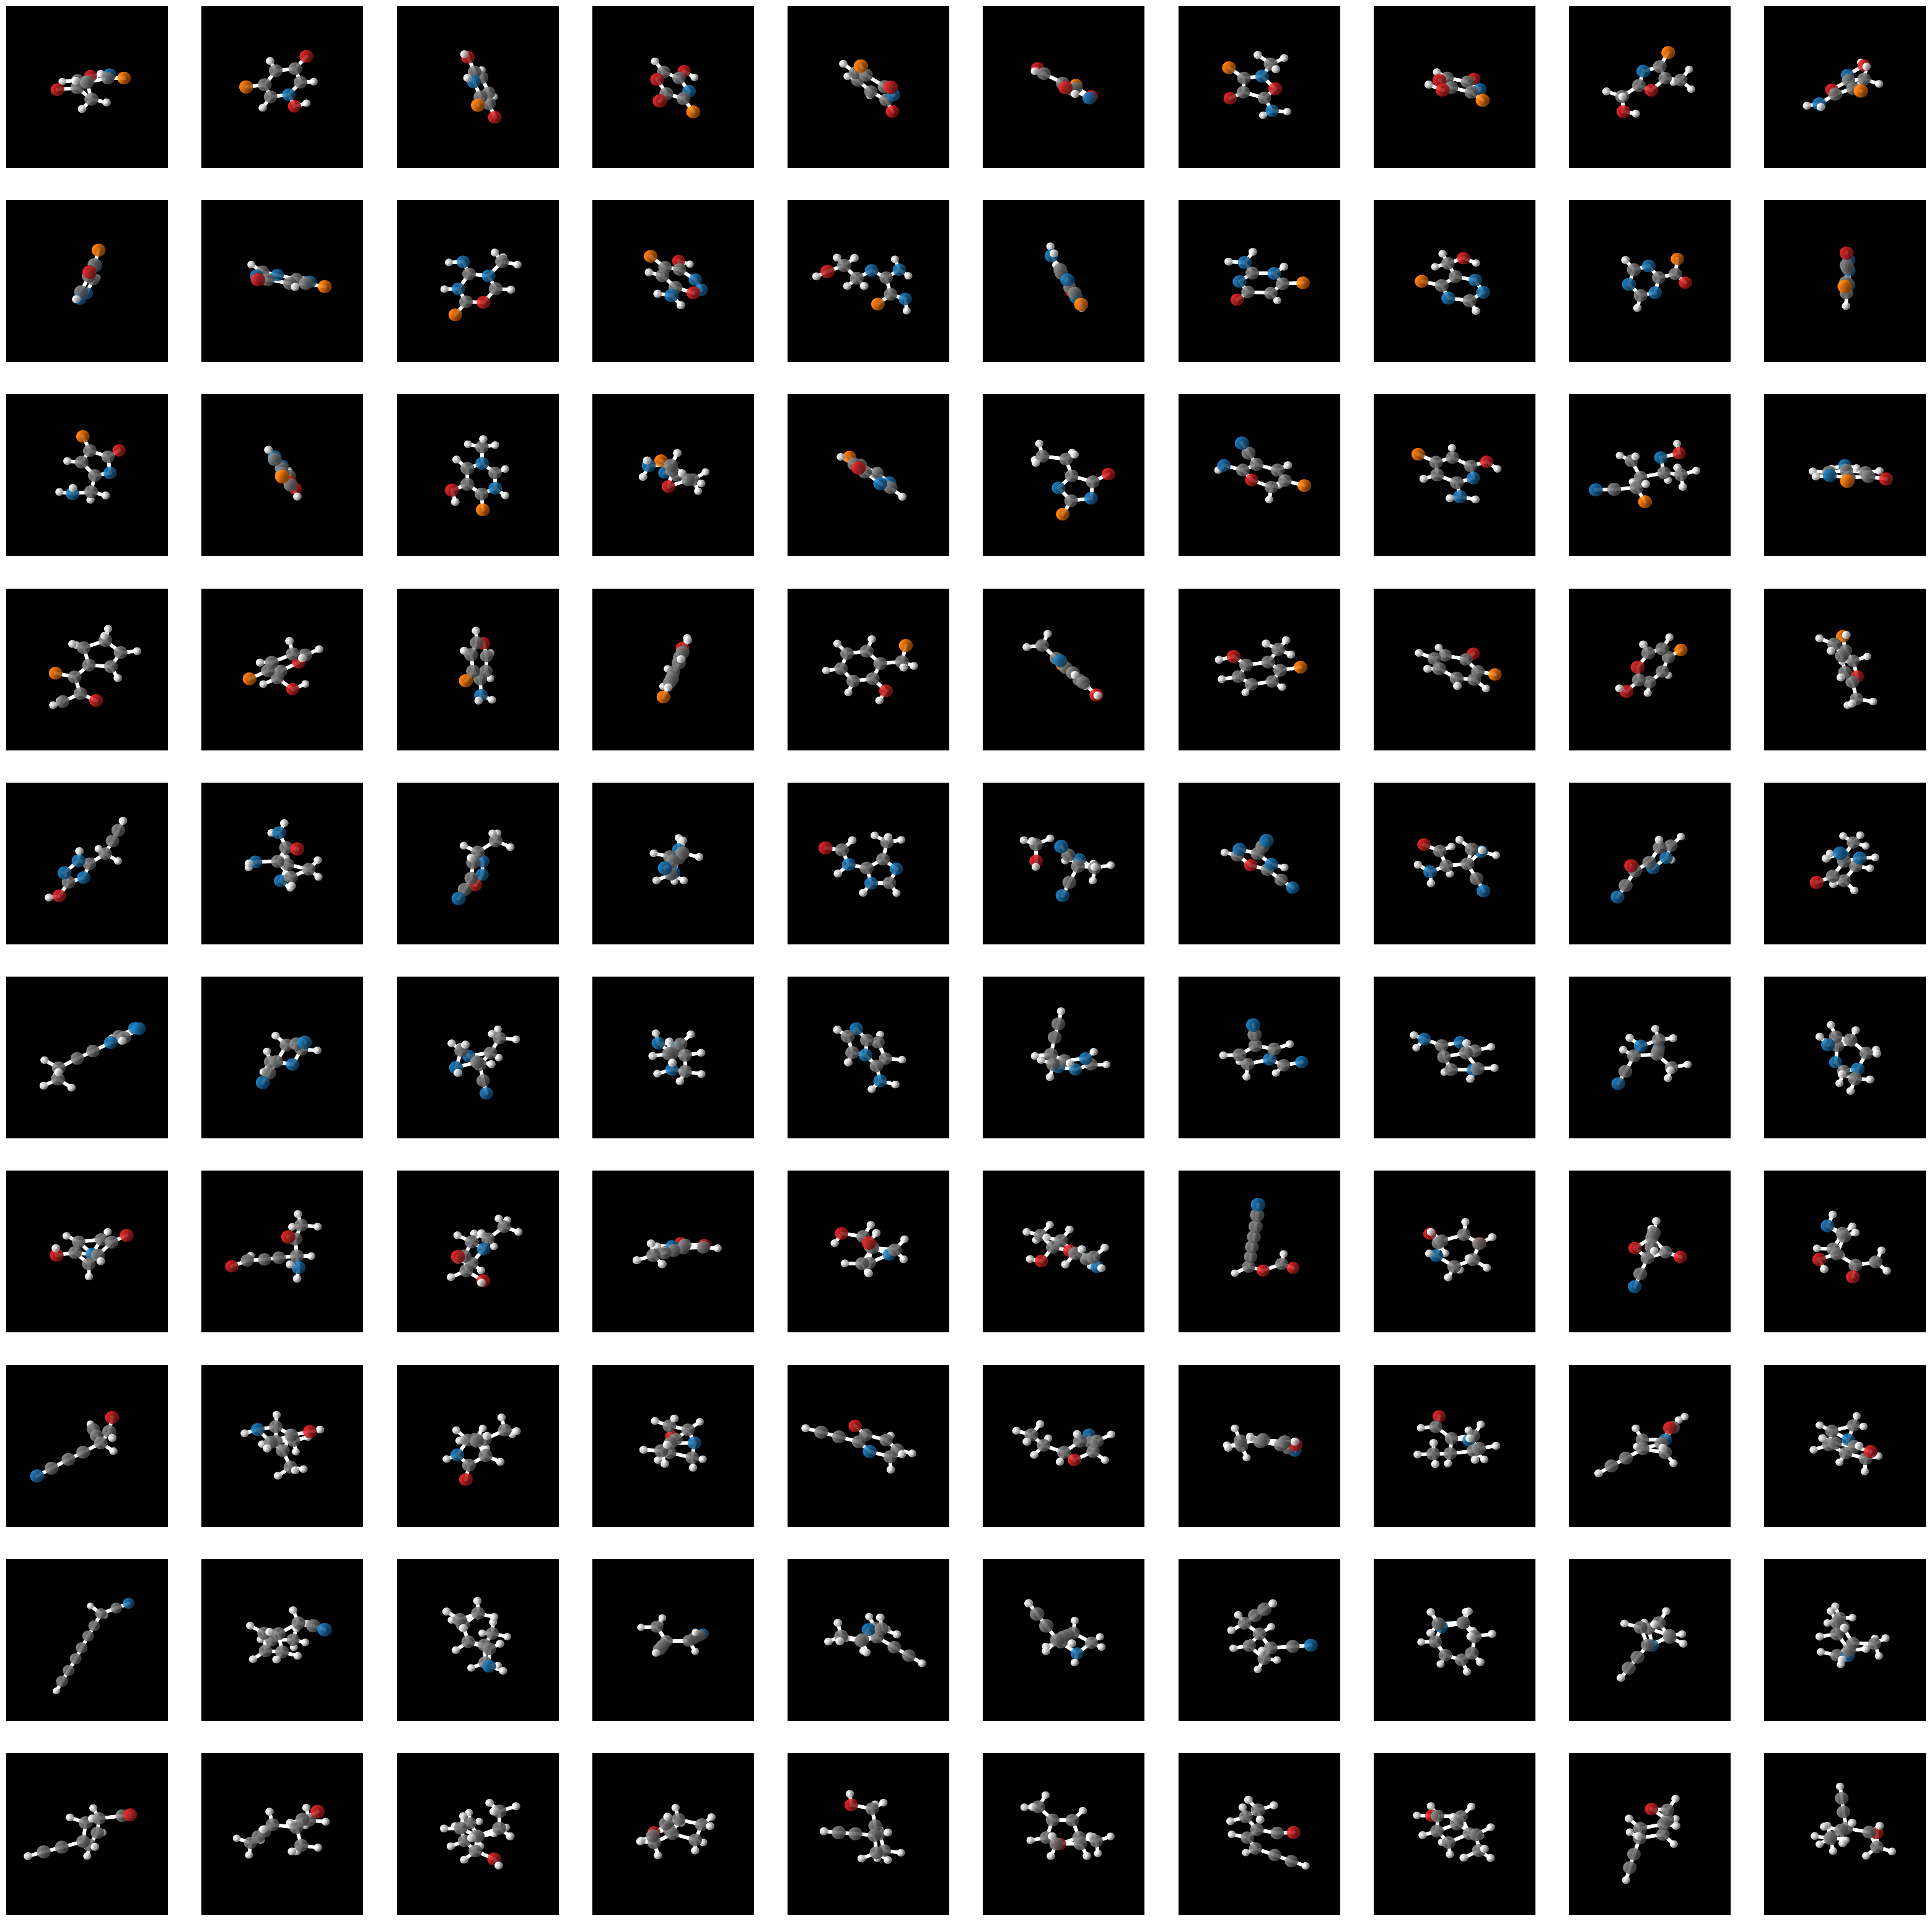
\includegraphics[width=\textwidth]{figs/tddm/cond_samples_image_bright.png}
    \caption{Samples generated by our model when conditional diffusion guidance is applied. Each row represents one task with task $1$ at the top, down to task $10$ at the bottom. For each task, $10$ samples are shown in each row.}
    \label{fig:tddm-CondSampleExamples}
\end{figure}

\begin{figure}
    \centering
    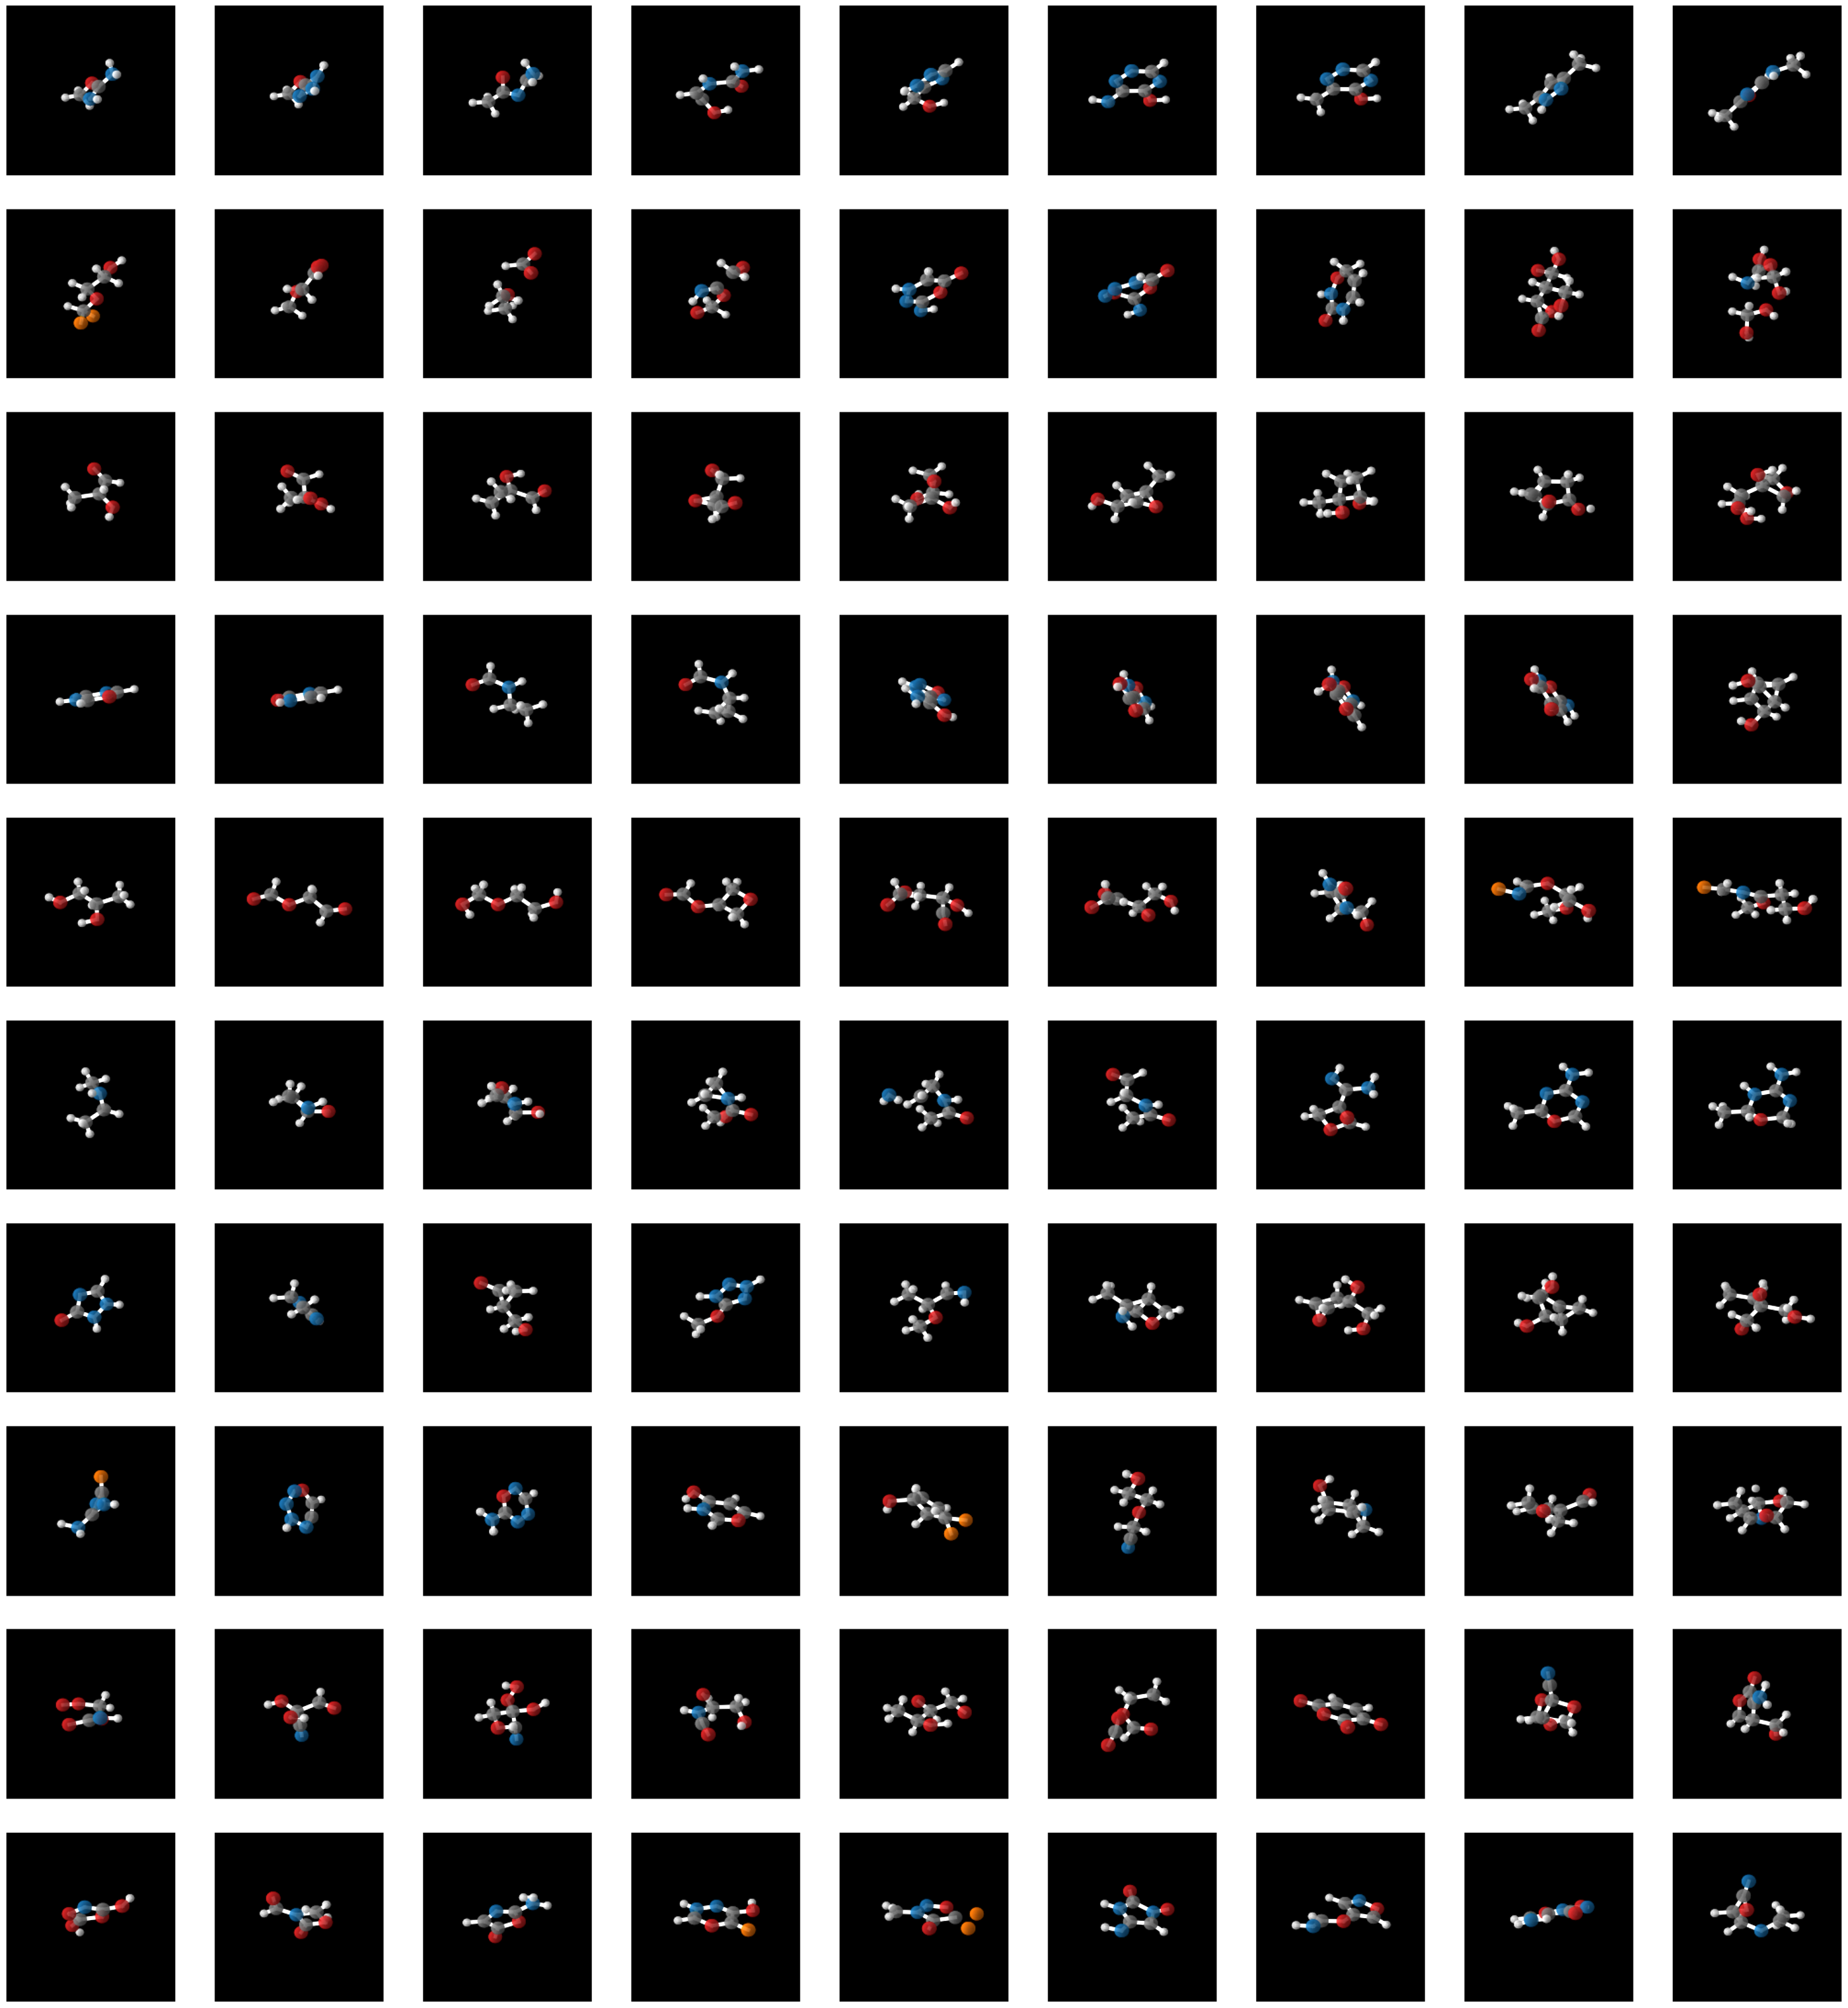
\includegraphics[width=\textwidth]{figs/tddm/interp_bright.png}
    \caption{Interpolations showing a sequence of generations for linearly increasing polarizability from $39 \, \text{Bohr}^3$ to $66 \, \text{Bohr}^3$ with fixed random noise. Each row shows an individual interpolation with $\text{Bohr}^3$ increasing from left to right.}
    \label{fig:tddm-apdxMoreInterps}
\end{figure}

\subsubsection{Ablations}
For our main model, we set $\forwardrate_{t < 0.1T} = 0$ to ensure that all dimensions are added with enough generation time remaining for the diffusion process to finalise all state values. To verify this setting, we compare its performance with $\forwardrate_{t<0.03T} = 0$ and $\forwardrate_{t<0.3T} = 0$. We show our results in \cref{tab:lowTablation}. We find that the $\forwardrate_{t<0.03T}=0$ setting to generate reasonable sample quality but incur some extra dimension error due to the generative process sometimes observing a lack of dimensions near $t=0$ and adding too many dimensions. We observed the same effect in the paper for when setting $\forwardrate_t$ to be constant for all $t$ in \cref{tab:cond_mol}. Further, the setting $\forwardrate_{t<0.3T}=0$ also results in increased dimension error due to there being less opportunity for the guidance model to supervise the number of dimensions. We find that $\forwardrate_{t<0.1T}=0$ to be a reasonable trade-off between these effects.
\begin{table}[ht]
\centering
\caption{Ablation of when to set the forward rate to $0$ on the conditional molecule generation task. We report dimension error as the average Hellinger distance between the generated and ground truth conditional dimension distributions as well as average sample quality metrics. Metrics are reported after 620k training iterations.}
\begin{tabular}{@{}lcccc@{}}
\toprule
Method & Dim.  Error & \% Atom stable & \% Molecule Stable & \% Valid \\ \midrule
$ \overrightarrow{\lambda}_{t < 0.03T} = 0$ & $0.227 {\scriptstyle \pm 0.16}$ & $91.5 {\scriptstyle \pm 3.7} $  & $56.5 {\scriptstyle \pm 9.8}$ & $72.0 {\scriptstyle \pm 11}$  \\
$ \overrightarrow{\lambda}_{t < 0.1T} = 0$ & $0.162 {\scriptstyle \pm 0.071}$ & $92.4 {\scriptstyle \pm 2.8}$ & $53.9 {\scriptstyle \pm 12}$ & $72.7 {\scriptstyle \pm 9.6}$ \\
$ \overrightarrow{\lambda}_{t < 0.3T} = 0$ & $0.266 {\scriptstyle \pm 0.11}$ & $92.0 {\scriptstyle \pm 3.2}$ & $53.5 {\scriptstyle \pm 13}$ & $66.6 {\scriptstyle \pm 12}$ \\
\bottomrule
\end{tabular}
\label{tab:lowTablation}
\end{table}

\subsubsection{Uniqueness and novelty metrics}
We here investigate sample diversity and novelty of our unconditional generative models. We measure uniqueness by computing the chemical graph corresponding to each generated sample and measure what proportion of the 10000 produced samples have a unique chemical graph amongst this set of 10000 as is done by \citet{hoogeboom2022equivariant}. We show our results in \cref{tab:uniqueness_and_novelty} and find our TDDM method to have slightly lower levels of uniqueness when compared to the fixed dimension diffusion model baseline. Measuring novelty on generative models trained on the QM9 dataset is challenging because the QM9 dataset contains an exhaustive enumeration of all molecules that satisfy certain predefined constraints~\citep{vignac2021top,hoogeboom2022equivariant}. Therefore, if a novel molecule is produced it means the generative model has failed to capture some of the physical properties of the dataset and indeed it was found by \citet{hoogeboom2022equivariant} that during training, as the model improved, novelty decreased. Novelty is therefore not typically included in evaluating molecular diffusion models. For completeness, we include the novelty scores in \cref{tab:uniqueness_and_novelty} as a comparison to the results presented in Appendix C of \citet{hoogeboom2022equivariant}. We find that our samples are closer to the statistics of the training dataset whilst still producing ‘novel’ samples at a consistent rate.
\begin{table}[ht]
     \centering
   \caption{Uniqueness and novelty metrics on unconditional molecule generation. We produce 10000 samples for each method and measure validity using RDKit. Uniquenss is judged as whether the chemical graph is unique amongst the 10000 produced samples. Amongst the valid and unique molecules, we then find the percentage that have a chemical graph not present in the training dataset.}
   \begin{tabular}{@{}lcccc@{}}
     \toprule
     Method & \% Valid  & \% Valid and Unique & \shortstack{Percentage of Valid and Unique \\ Molecules that are Novel } \\ \midrule
     FDDM [8] & $91.9$ & $90.7$ & $65.7$ \\ \midrule
     TDDM (ours) & $92.3$ & $89.9$ & $53.6$ \\
     TDDM, const $\smash{\overrightarrow{\lambda}_t}$ & $86.7$ & $84.4$ & $56.9$ \\
     TDDM, $\overrightarrow{\lambda}_{t<0.9T} = 0$ & $89.4$ & $86.1$ & $51.3$ \\
     TDDM w/o Prop. 3 & $87.1$ & $85.9$ & $63.3$ \\ \bottomrule
   \end{tabular}
   \label{tab:uniqueness_and_novelty}
\end{table}




\subsection{Video}
\subsubsection{Dataset}
We used the VP$^2$ benchmark, which consists of 35\,000 videos, each 35 frames long. The videos are evenly divided among seven tasks, namely: \texttt{push \{red, green, blue\} button, open \{slide, drawer\}, push \{upright block, flat block\} off table}. The 5000 videos for each task were collected using a scripted task-specific policy operating in the RoboDesk environment~\citep{kannan2021robodesk}. They sample an action vector at every step during data generation by adding i.i.d.\ Gaussian noise to each dimension of the action vector output by the scripted policy. For each task, they sample 2500 videos with noise standard deviation 0.1 and 2500 videos with standard deviation 0.2. We filter out the lower-quality trajectories sampled with noise standard deviation 0.2, and so use only the 17\,500 videos (2500) per task with noise standard deviation 0.1. We convert these videos to $32\times32$ resolution and then, so that the data we train on has varying lengths, we create each training example by sampling a length $l$ from a uniform distribution over $\{2,\ldots,35\}$ and then taking a random $l$-frame subset of the video.

\subsubsection{Forward process}
The video domain differs from molecules in two important ways. The first is that videos cannot be reasonably treated as a permutation-invariant set. This is because the order of the frames matters. Secondly, generating a full new component for the molecules with a single pass autoregressive network is feasible, however, a component for the videos is a full frame which is challenging for a single pass autoregressive network to generate. We design our forward process to overcome these challenges.

We define our forward process to delete frames in a random order. This means that during generation, frames can be generated in any order in the reverse process, enabling more conditioning tasks since we can always ensure that whichever frames we want to condition on are added first. Further, we use a non-isotropic noise schedule by adding noise just to the frame that is about to be deleted. Once it is deleted, we then start noising the next randomly chosen frame. This is so that, in the reverse direction, when a new frame is added, it is simply Gaussian noise. Then the score network will fully denoise that new frame before the next new frame is added. We now specify exactly how our forward process is constructed.

We enable random-order deletion by applying an initial shuffling operation occurring at time $t=0$. Before this operation, we represent the video $\rvx$ as an ordered sequence of frames, $\rvx_0=[\rvx_1,\rvx_2,\ldots,\rvx_{n_0}]$. During shuffling, we sample a random permutation $\pi$ of the integers $1,\ldots,n_0$. Then the frames are kept in the same order, but annotated with an index variable so that we have 
\begin{equation}
    \rvx_{0^+}=[(\rvx_{0}^{(1)}, \pi(1)), (\rvx_{0}^{(2)}, \pi(2)), \ldots, (\rvx^{(n_0)}_{0}, \pi(n_0))].
\end{equation}

We will run the forward process from $t=0$ to $t = 100N$. We will set the forward rate such we delete down from $n_t$ to $n_t - 1$ at time $(N-n_t+1)100$. This is achieved heuristically by setting
\begin{equation}
    \forwardrate_t(n_t) = \begin{cases}
        0 & \text{for } t < (N-n_t+1)100, \\
        \infty & \text{for }  t \geq (N-n_t + 1) 100.
    \end{cases} 
\end{equation}
We can see that at time $t = (N - n_t + 1)100$ we will quickly delete down from $n_t$ to $n_t-1$ at which point $\forwardrate_t(n_t)$ will become $0$ thus stopping deletion until the process arrives at the next multiple of $100$ in time. When we hit a deletion event, we delete the frame from $\mX_t$ that has the current highest index variable $\pi(n)$. In other words
\begin{equation}
    \delidxdist(i | \mX_t) = \begin{cases}
        1 & \text{for } n_t = \rvx_{t}^{(i)}[2], \\
        0 & \text{otherwise}
    \end{cases}    
\end{equation}
where we use $\rvx_{t}^{(i)}[2]$ to refer to the shuffle index variable for the $i$th current frame in $\rvx_{t}$.


We now provide an example progression of the forward deletion process. Assume we have $n_0=4$, $N=5$ and sample a permutation such that $\pi(1)=3, \pi(2)=2, \pi(3)=4$, and $\pi(4)=1$. Initially the state is augmented to include the shuffle index. Then the forward process progresses from $t=0$ to $t=500$ with components being deleted in descending order of the shuffle index
\begin{align}
    \rvx_{0^+}&=[(\rvx^{(1)}_{t}, 3), (\rvx^{(2)}_{t}, 2), (\rvx^{(3)}_{t}, 4), (\rvx^{(4)}_{t}, 1)]\\
    \rvx_{100^+} &= [(\rvx^{(1)}_{t}, 3), (\rvx^{(2)}_{t}, 2), (\rvx^{(3)}_{t}, 4), (\rvx^{(4)}_{t}, 1)]\\
    \rvx_{200^+} &= [(\rvx^{(1)}_{t}, 3), (\rvx^{(2)}_{t}, 2), (\rvx^{(4)}_{t}, 1)]\\
    \rvx_{300^+} &= [(\rvx^{(2)}_{t}, 2), (\rvx^{(4)}_{t}, 1)]\\
    \rvx_{400^+} &= [(\rvx^{(4)}_{t}, 1)]\\
\end{align}
In this example, due to the random permutation sampled, the final video frame remained after all others had been deleted. Note that the order of frames is preserved as we delete frames in the forward process although the spacing between them can change as we delete frames in the middle.


Between jumps, we use a noising process to add noise to frames. The noising process is non-isotropic in that it adds noise to different frames at different rates such that the a frame is noised only in the time window immediately preceding its deletion. For component $i \in [1, \dots, n_t]$, we set the forward noising process such that $p_{t|0}(\rvx_t^{(i)} | \rvx_0^{(i)}, M_t) = \mathcal{N}(\rvx_t^{(i)}; \rvx_0^{(i)}, \sigma_t(\rvx_t^{(i)})^2)$ where $\rvx_0^{(i)}$ is the clean frame corresponding to $\rvx_t^{(i)}$ as given by the mask $M_t$ and $\sigma_t(\rvx_t^{(i)})$ follows
\begin{equation}
    \sigma_t(\rvx_t^{(i)}) = \begin{cases}
        0 & \text{for } t < (N - \rvx_t^{(i)}[2]) 100,\\
        100 & \text{for } t > (N - \rvx_t^{(i)}[2]) 100,\\
        t - (N - \rvx_t^{(i)}[2])100 & \text{for } (N - \rvx_t^{(i)}[2])100 \leq t \leq (N - \rvx_t^{(i)}[2]+1) 100
    \end{cases}
\end{equation}
where we again use $\rvx_t^{(i)}[2]$ for the shuffle index of component $i$. This is the VE-SDE from \citet{song2020score} applied to each frame in turn. We note that we only add noise to the state values on not the shuffle index itself. The SDE parameters that result in the VE-SDE are $\forwarddrift_t = 0$ and $\forwarddiffcoeff_t = \sqrt{2t - 2(N - \rvx_t^{(i)}[2])100}$.



\subsubsection{Sampling the reverse process}

When $t$ is not at a multiple of 100, the forward process is purely adding Gaussian noise, and so the reverse process is also purely operating on the continuous dimensions. We use the Heun sampler proposed by \citet{karras2022elucidating} to update the continuous dimensions in this case, and also a variation of their discretisation of $t$ - specifically to update from e.g. $t=600$ to $t=500$, we use their discretisation of $t$ as if the maximum value was 100 and then offset all values by $500$. 

To invert the dimension deletion process, we can use \cref{prop:backwardrateparam} to derive our reverse dimension generation process. We re-write our parameterised $\backwardrate_t^\theta$ using \cref{prop:backwardrateparam} as 
\begin{equation}
    \backwardrate_t^\theta(\mX_t) = \forwardrate_t(n_t + 1) \mathbb{E}_{p_{0|t}^\theta(n_0 | \mX_t)} \left[ \frac{p_{t|0}(n_t + 1 | n_0)}{p_{t|0}(n_t | n_0)}\right]
\end{equation}
At each time multiple of 100 in the reverse process, we will have an opportunity to add a component. At this time point, we estimate the expectation with a single sample $n_0 \sim p_{0|t}^\theta(n_0 | \mX_t)$. If $n_0 > n_t$ then $\backwardrate_t^\theta(\mX_t) = \infty$. The new component will then be added at which point $\backwardrate_t^\theta(\mX_t)$ becomes $0$ for the remainder of this block of time due to $n_t$ becoming $n_t+1$. If $n_0 = n_t$ then $\backwardrate_t^\theta(\mX_t) = 0$ and no new component is added. $\backwardrate_t^\theta(\mX_t)$ will continue to be $0$ for the remainder of the reverse process once an opportunity to add a component is not used.

When a new frame is added, we use $\autonet_t^\theta(\yadd, i | \mX_t)$ to decide where the frame is added and its initial value. Since when we delete a frame it is fully noised, $\autonet_t^\theta(\yadd, i | \mX_t)$ can simply predict Gaussian noise for the new frame $\yadd$. However, $\autonet_t^\theta(\yadd, i | \mX_t)$ will still learn to predict a suitable location $i$ to place the new frame such that reverse process is the reversal of the forward.

We give an example simulation from the reverse generative process in \cref{fig:tddm-examplevideoreverse}.

\begin{figure}
    \centering
    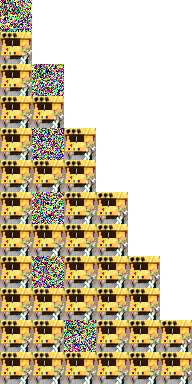
\includegraphics[width=6cm]{figs/tddm/short-obs-32.png}
    \caption{An example simulation of the reverse generative process conditioned on the first and last frame. Note how the process first adds a new frame and then fully denoises it before adding the next frame. Since the first and last frame are very similar, the process produces a short video.}
    \label{fig:tddm-examplevideoreverse}
\end{figure}




\subsubsection{Network architecture}
Our video diffusion network architecture is based on the U-net used by \citet{harvey2022flexible}, which takes as input the index of each frame within the video, and uses the differences between these indices to control the interactions between frames via an attention mechanism. Since, during generation, we do not know the final position of each frame within the $\rvx_0$, we instead pass in its position within the ordered sequence $\rvx_t$.

One further difference is that, since we are perform non-isotropic diffusion, the standard deviation of the added noise will differ between frames. We adapt to this by performing preconditioning, and inputting the timestep embedding, separately for each frame $\rvx_t^{(i)}$ based on $\sigma_t(\rvx_t^{(i)})$ instead of basing them on the global diffusion timestep $t$. Our timestep embedding and pre- and post-conditioning of network inputs/outputs are as suggested by \citet{karras2022elucidating}, other than being done on a per-frame basis. The architecture from \citet{harvey2022flexible} with these changes applied then gives us our score network $\rvs_\theta$.

While it would be possible to train a single network that estimates the score and all quantities needed for modelling jumps, we chose to train two separate networks in order to factorise our exploration of the design space. These were the score network $\rvs_\theta$, and the rate and index prediction network modelling $p_{0|t}^\theta(n_0 | \mX_t)$ and $\autonet_t^\theta(i | \mX_t)$. The rate and index prediction network is similar to the first half of the score network, in that it uses all U-net blocks up to and including the middle one. We then flatten the $512\times4\times4$ hidden state for each frame after this block such that, for an $n_t$ frame input, we obtain a $n_t \times 8192$ hidden state. These are fed through a 1D convolution with kernel size $2$ and zero-padding of size $1$ on each end, reducing the hidden state to $(n_t+1) \times 128$, which is in turn fed through a ReLU activation function. This hidden state is then fed into three separate heads. One head maps it to the parameters of $\autonet_t^\theta(i | \mX_t)$ via a 1D convolution of kernel size 3. The output of size $(n_t+1)$ is fed through a softmax to provide the categorical distribution $\autonet_t^\theta(i | \mX_t)$. The second head averages the hidden state over the ``frame'' dimension, producing a $128$-dimensional vector. This is fed through a single linear layer and a softmax to parameterise $p_{0|t}^\theta(n_0 | \mX_t)$. Finally, the third head consists of a 1D convolution of kernel size 3 with 35 output channels. The $(n_t+1)\times35$ output is fed through a softmax to parameterise distributions over the number of frames that were deleted from $\mX_0$ which came before the first in $\rvx_t$, the number of frames from $\mX_0$ which were deleted between each pair of frames in $\rvx_t$, and the number deleted after the last frame in $\rvx_t$. We do not use this head at inference-time but found that including it improved the performance of the other heads by helping the network learn better representations. 

For a final performance improvement, we note that under our forward process there is only ever one ``noised'' frame in $\rvx_t$, while there are sometimes many clean frames. Since the cost of running our architecture scales with the number of frames, running it on many clean frames may significantly increase the cost while providing little improvement to performance. We therefore only feed into the architecture the ``noised'' frame, the two closest ``clean'' frames before it, and the two closest ``clean'' frames after it. See our released source code for the full implementation of this architecture.

\subsubsection{Training}
To sample $t$ during training, we adapt the log-normal distribution suggested by \citet{karras2022elucidating} in the context of isotropic diffusion over a single image. To apply it to our non-isotropic video diffusion, we first sample which frames have been deleted, which exist with no noise, and which have had noise added, by sampling the timestep from a uniform distribution and simulating our proposed forward process. We then simply change the noise standard deviation for the noisy frame, replacing it with a sample from the log-normal distribution. The normal distribution underlying our log-normal has mean $-0.6$ and standard deviation $1.8$. 
%
This can be interpreted as sampling the timestep from a mixture of log-normal distributions, $\frac{1}{N}\sum_{i=0}^{N-1} \mathcal{LN}(t-100i; -0.6, 1.8^2)$. Here, the mixture index $i$ can be interpreted as controlling the number of deleted frames.

We use the same loss weighting as \citet{karras2022elucidating} but, similarly to our use of preconditioning, compute the weighting separately for each frame $\rvx_t^{(i)}$ as a function of $\sigma_t(\rvx_t^{(i)})$ to account for the non-isotropic noise.

\subsubsection{Perceptual quality metrics}
We now verify that our reverse process does not have any degradation in quality during the generation as more dimensions are added. We generate 10000 videos and throw away the 278 that were sampled to have only two frames. We then compute the FID score for individual frames in each of the remaining 9722 videos. We group together the scores for all the first frames to be generated in the reverse process and then for the second frame to be generated and so on. We show our results in \cref{tab:fid-by-insertion-order}. We find that when a frame is inserted has no apparent effect on perceptual quality and conclude that there is no overall degradation in quality as our sampling process progresses. We note that the absolute value of these FID scores may not be meaningful due to the RoboDesk dataset being far out of distribution for the Inception network used to calculate FID scores. We can visually confirm good sample quality from \cref{fig:tddm-video_example}.
\begin{table}[ht]
\centering
\caption{FID for video frames grouped by when they were inserted during sampling.}
\begin{tabular}{p{1.5cm}p{1.5cm}p{1.5cm}|p{1.5cm}p{1.5cm}p{1.5cm}}
\toprule
1st & 2nd & 3rd & 3rd last & 2nd last & last \\
\midrule
34.2 & 34.9 & 34.7 & 34.2 & 34.1 & 34.4 \\
\bottomrule
\label{tab:fid-by-insertion-order}
\end{tabular}
\end{table}